\documentclass[conference]{IEEEtran}
\IEEEoverridecommandlockouts
% The preceding line is only needed to identify funding in the first footnote. If that is unneeded, please comment it out.
\usepackage{cite}
\usepackage{amsmath,amssymb,amsfonts}
\usepackage{algorithmic}
\usepackage{graphicx}
\usepackage{textcomp}
\usepackage{xcolor}
\def\BibTeX{{\rm B\kern-.05em{\sc i\kern-.025em b}\kern-.08em
    T\kern-.1667em\lower.7ex\hbox{E}\kern-.125emX}}
\begin{document}

\title{A Comparison of Different Computer Vision Methods and Algorithms for the
    Classification of Aquatic Macroinvertebrates\\
{\footnotesize \textsuperscript{*}A Computer Vision project for the Department
of Engineering at Aarhus University}
}

\author{\IEEEauthorblockN{Th\'{e}o Morales}
\IEEEauthorblockA{\textit{MSc. Student of Computer Engineering} \\
\textit{Faculty of Science and Technology, Department of Engineering}\\
Aarhus University, Denmark \\
theo.martin.morales@post.au.dk}
}

\maketitle

\begin{abstract}
    Measuring water quality in natural environments can be a difficult problem to tackle. One of the ways of assessing the quality of fresh water in such environment is to observe and analyse the different aquatic macroinvertebrates that live in it. Using modern Computer Vision methods to do so is inherently more efficient, in terms of time and cost, than relying on the sole human expertise. Developing proper techniques in order to achieve similar, if not better, results than manual observation and analysis is the ultimate goal of this research. In this paper, a subset of the original dataset is used to conduct independent research on different image classification algorithms, and to compare several common ones with the state of the art Convolutional Neural Networks.
\end{abstract}

\begin{IEEEkeywords}
    CNN, Deep Neural Network, image classification, computer vision, machine learning
\end{IEEEkeywords}

\section{Introduction}
Ensuring the quality of water sources is an important task for the good of a human population, as well as the one of its surrounding ecosystem. Water can be infected with all sorts of bacteria, but can also contain a significant amount of micro-organisms that wouldn't be suited for human consumption, but nevertheless being part of a natural aquatic ecosystem that could be seen as a gage of quality and sanity.

However, measuring such concept isn't as trivial as what is commonly done with regular metrics, and it requires more reasoning and analysing than most standard measures in the scientific domain do. This study focuses on the analysis of known aquatic macroinvertebrates, which are part of aquatic ecosystems in water sources, and their automated classification using a machine learning approach. The end goal is to provide a reliable method for this task, that would ultimately surpass the human expertise in the field. In this paper, a set of well known and commonly used machine learning and computer vision methods are presented, and their results are compared and discussed after application on the dataset; the famous state-of-the-art Convolutional Neural Network will be used as a reference point in the benchmark.

\section{Dataset}

\subsection{Dataset presentation}
The provided dataset contains a subset of the whole dataset from the original research paper that this project leans on. It contains \textbf{5830} \emph{Training} samples, \textbf{2298} \emph{Validation} samples, and \textbf{3560} \emph{Test} samples. These sets are given in two forms:
\begin{itemize}
    \item the original images in color with a \textbf{\textsc{28x28}} pixel dimension, in the JPEG format
    \item the abstract representations of the images as a set of 4096-dimensional vectors (available inn \emph{CSV}, \emph{Matlab} and \emph{text} formats), obtained after feeding the base pictures to a CNN, pre-trained on the training dataset
\end{itemize}

\begin{figure}[h]
    \centering
        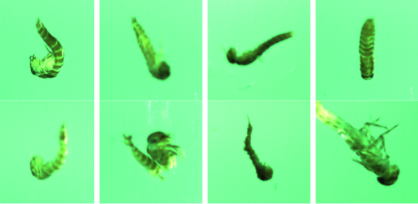
\includegraphics[height=4cm]{sample_macrobitches}
    \caption{Four samples from Baetis niger (top) and Ameletus inopinatus (bottom) classes.}
\end{figure}

It goes without saying that each set also comes with its corresponding labels definition (available in \emph{CSV}, \emph{Matlab} and \emph{text} formats), except for the \emph{Test} dataset which labels, of course, need to be "guessed" by the classifier.


\subsection{Dataset pre-processing}
One important thing to mention is that the given JPEG pictures are already cropped to focus on the target object, thus minimizing the need for data pre-processing in some cases where not much needs to be done. For example, with computer vision methods such as \emph{SIFT} or \emph{HOG} features classification, a minimal amount of data preparation is necessary for the algorithms to be effective: vector normalization is often just enough. In this study, the \emph{Feature Scaling} normalization technique is used, in order to bring all the dataset's values into the range [0,1]:

\begin{equation}
    x_{new}=\frac{x_i-\min(x)}{\max(x)-\min(x)}
\end{equation}

With $x_i$ being the current value of the sample (a vector in this case), $\min(x)$ being the minimum value of the current dataset, and $\max(x)$ being the maximum value of the same dataset. This technique is useful when the classifier is computing a lot of multiplications, since it greatly reduces the difference between the two products when the multiplied values are very close to each other, thus restraining the scatter of the samples.

Data standardization can also be used in order to improve the classification results, by reducing the mean and unit variance to zero, using the following equation:

\begin{equation}
    x_{new}=\frac{x_i-\mu}{\sigma}
\end{equation}

Where $\mu$ is the mean of the dataset, and $\sigma$ is the variance of the same dataset. 

Concerning the Convolutional Neural Networks approach, a few more things have to be taken into consideration. In this project, a pre-trained CNN is used for fine-tuning over this dataset, meaning that the weights of the convolution layers are unchanged. This implies that the images fed into the network must be the same size as the ones it has been trained with. Without going into further details (more will be explained in the appropriate section), the JPEG images for this dataset had to be scaled up to match the network's input layer (\textsc{299x299} pixels), and some distortion is applied to the \emph{Training} images. Other than that, each image is normalized as previously explained.

\subsection{Dataset augmentation}
As stated above, \emph{Dataset Augmentation} is a process that is only applied to images used for a Convolutional Neural Network training phase, because it is the classifier that takes the most advantage of the three color channels of an image. It is only useful to augment the \emph{Training} sample images, since those are the only ones that will help the classifier to learn.
The \emph{Python} script provided by \emph{Tensorflow} for \emph{Inception Resnet v2} tales care of distorting images in order to augment the data set, to ultimately make the network invariant to aspects of the image that do not effect the label. Since the aspect ratio is not respected, and since the resizing method changes depending on the running thread number, the resizing operation may distort the images in a first place. Secondly, each image is randomly flipped horizontally. Finally, the colors are randomly distorted in four different ways.

\section{Methods and algorithms}
Classifying images of such similar shapes can be a difficult task to solve as a machine learning problem, and that is why several algorithms and methods must be applied on the same dataset in order to have a certain order of comparison to be able to conclude useful deductions.
Finding the right method to properly classify the dataset is the ultimate goal, but before simply going for the state-of-the-art CNN, it is best to study the well known methods and understand why one performs better than an other, in an attempt to apply the best possible approach.

The following algorithms have been applied and compared against each other:
\begin{itemize}
    \item \textbf{Multi Layer Perceptron Neural Network}
    \item \textbf{Pre-Trained Convolutional Neural Network}
    \item \textbf{Support Vector Machine with Bag Of Features}
    \item \textbf{Nearest Neighbour with Bag Of Features}
\end{itemize}

Those algorithms were implemented in \emph{Python 3}, with the help of the great libraries \emph{Tensorflow} and \emph{OpenCV}. In the following section, they will be presented and explained thoroughly, after what their results will be compared on the same basis. \emph{Note that the given accuracy corresponds to the validation accuracy, and that it may vary if measured on the test dataset.}

\subsection{Multi Layer Perceptron Neural Network}
    Famously known for being able to optimize a large range of cost functions, the MLP Neural Network does not need to be presented. The thing that makes it a very good candidate against the convolutional type is its fully-connected architecture, that is part of the actual CNN architecture as being the last "step".
Since the feature vectors provided in the dataset were produced by a CNN, it should be intuitive to think that feeding those into an independent MLP would produce rather similar results, and that is why it can be assumed that both scores should be close to each other.

The MLP has been trained from scratch using different architecures for the hidden layers, and with two different optimizers: \emph{Adam} and \emph{Stochastic Gradient Descent}, both with similar learning rates. Different results can be observed after tinkering with the hyperparameters, before optaining what is to be considered the optimal configuration for the last row of the table:

\begin{table}[htbp]
\caption{Multi Layer Perceptron: \\ Hyperparameters and Configurations}
\begin{center}
\begin{tabular}{|c|c|c|c|}
\hline
\multicolumn{3}{|c|}{\textbf{Hyperparameters}}&\textbf{Final} \\
\cline{1-3} 
\textbf{\textit{Hidden Neurons}}& \textbf{\textit{Learn. Rate}}& \textbf{\textit{Batch Size}} & \textbf{\textit{Accuracy}} \\
\hline
2048:1024& 0.0018 & 50 & 72\% \\
\hline
\end{tabular}
\label{tab1}
\end{center}
\end{table}


\subsection{Pre-Trained Convolutional Neural Network}
    As previously explained, using a pre-trained Convolutional Neural Network has the big advantage of providing well-performing convolution layers, which play the biggest part in image classification for such a type of neural network.
The chosen CNN is \emph{Inception Resnet V2}, that is part of \emph{Tensorflow-slim}'s research architectures and one of the top performing CNNs out there, according to [INSERT REF TO GITHUB REPO PLEASE].

A checkpoint of that network, containing all the weights and biases, was downloaded and used to transfer the learning of the model, by keeping the convolution layers's weights but dropping the fully-connected layers's ones, in order to fine-tune the network with the macroinvertebrates dataset.
This was done fairly easily thanks to the good usability of the framework, and as stated above, a pre-processing script is provided for the images to be fitted into the network's input configuration.

This method is allegedly the best in the field, and if used well, can yield impressive results of accuracy above 95\%. However, since the computation of such network (especially on a large model like \emph{Inception}) is very slow and requires a recent GPU with CUDA capabilities, it has been hard to obtain decent results that would support the theory.

\subsection{Support Vector Machine with Bag Of Features}

\subsection{Nearest Neighbour with Bag Of Features}


\subsection{Some Common Mistakes}\label{SCM}

\subsection{Authors and Affiliations}
\textbf{The class file is designed for, but not limited to, six authors.} A 
minimum of one author is required for all conference articles. Author names 
should be listed starting from left to right and then moving down to the 
next line. This is the author sequence that will be used in future citations 
and by indexing services. Names should not be listed in columns nor group by 
affiliation. Please keep your affiliations as succinct as possible (for 
example, do not differentiate among departments of the same organization).

\subsection{Identify the Headings}
Headings, or heads, are organizational devices that guide the reader through 
your paper. There are two types: component heads and text heads.

Component heads identify the different components of your paper and are not 
topically subordinate to each other. Examples include Acknowledgments and 
References and, for these, the correct style to use is ``Heading 5''. Use 
``figure caption'' for your Figure captions, and ``table head'' for your 
table title. Run-in heads, such as ``Abstract'', will require you to apply a 
style (in this case, italic) in addition to the style provided by the drop 
down menu to differentiate the head from the text.

Text heads organize the topics on a relational, hierarchical basis. For 
example, the paper title is the primary text head because all subsequent 
material relates and elaborates on this one topic. If there are two or more 
sub-topics, the next level head (uppercase Roman numerals) should be used 
and, conversely, if there are not at least two sub-topics, then no subheads 
should be introduced.

\subsection{Figures and Tables}
\paragraph{Positioning Figures and Tables} Place figures and tables at the top and 
bottom of columns. Avoid placing them in the middle of columns. Large 
figures and tables may span across both columns. Figure captions should be 
below the figures; table heads should appear above the tables. Insert 
figures and tables after they are cited in the text. Use the abbreviation 
``Fig.~\ref{fig}'', even at the beginning of a sentence.

\begin{table}[htbp]
\caption{Table Type Styles}
\begin{center}
\begin{tabular}{|c|c|c|c|}
\hline
\textbf{Table}&\multicolumn{3}{|c|}{\textbf{Table Column Head}} \\
\cline{2-4} 
\textbf{Head} & \textbf{\textit{Table column subhead}}& \textbf{\textit{Subhead}}& \textbf{\textit{Subhead}} \\
\hline
copy& More table copy$^{\mathrm{a}}$& &  \\
\hline
\multicolumn{4}{l}{$^{\mathrm{a}}$Sample of a Table footnote.}
\end{tabular}
\label{tab1}
\end{center}
\end{table}

\begin{figure}[htbp]
\centerline{\includegraphics{fig1.png}}
\caption{Example of a figure caption.}
\label{fig}
\end{figure}

Figure Labels: Use 8 point Times New Roman for Figure labels. Use words 
rather than symbols or abbreviations when writing Figure axis labels to 
avoid confusing the reader. As an example, write the quantity 
``Magnetization'', or ``Magnetization, M'', not just ``M''. If including 
units in the label, present them within parentheses. Do not label axes only 
with units. In the example, write ``Magnetization (A/m)'' or ``Magnetization 
\{A[m(1)]\}'', not just ``A/m''. Do not label axes with a ratio of 
quantities and units. For example, write ``Temperature (K)'', not 
``Temperature/K''.

\section*{Acknowledgment}

The preferred spelling of the word ``acknowledgment'' in America is without 
an ``e'' after the ``g''. Avoid the stilted expression ``one of us (R. B. 
G.) thanks $\ldots$''. Instead, try ``R. B. G. thanks$\ldots$''. Put sponsor 
acknowledgments in the unnumbered footnote on the first page.

\section*{References}

Please number citations consecutively within brackets \cite{b1}. The 
sentence punctuation follows the bracket \cite{b2}. Refer simply to the reference 
number, as in \cite{b3}---do not use ``Ref. \cite{b3}'' or ``reference \cite{b3}'' except at 
the beginning of a sentence: ``Reference \cite{b3} was the first $\ldots$''

Number footnotes separately in superscripts. Place the actual footnote at 
the bottom of the column in which it was cited. Do not put footnotes in the 
abstract or reference list. Use letters for table footnotes.

Unless there are six authors or more give all authors' names; do not use 
``et al.''. Papers that have not been published, even if they have been 
submitted for publication, should be cited as ``unpublished'' \cite{b4}. Papers 
that have been accepted for publication should be cited as ``in press'' \cite{b5}. 
Capitalize only the first word in a paper title, except for proper nouns and 
element symbols.

For papers published in translation journals, please give the English 
citation first, followed by the original foreign-language citation \cite{b6}.

\begin{thebibliography}{00}
\bibitem{b1} G. Eason, B. Noble, and I. N. Sneddon, ``On certain integrals of Lipschitz-Hankel type involving products of Bessel functions,'' Phil. Trans. Roy. Soc. London, vol. A247, pp. 529--551, April 1955.
\bibitem{b2} J. Clerk Maxwell, A Treatise on Electricity and Magnetism, 3rd ed., vol. 2. Oxford: Clarendon, 1892, pp.68--73.
\bibitem{b3} I. S. Jacobs and C. P. Bean, ``Fine particles, thin films and exchange anisotropy,'' in Magnetism, vol. III, G. T. Rado and H. Suhl, Eds. New York: Academic, 1963, pp. 271--350.
\bibitem{b4} K. Elissa, ``Title of paper if known,'' unpublished.
\bibitem{b5} R. Nicole, ``Title of paper with only first word capitalized,'' J. Name Stand. Abbrev., in press.
\bibitem{b6} Y. Yorozu, M. Hirano, K. Oka, and Y. Tagawa, ``Electron spectroscopy studies on magneto-optical media and plastic substrate interface,'' IEEE Transl. J. Magn. Japan, vol. 2, pp. 740--741, August 1987 [Digests 9th Annual Conf. Magnetics Japan, p. 301, 1982].
\bibitem{b7} M. Young, The Technical Writer's Handbook. Mill Valley, CA: University Science, 1989.
\end{thebibliography}
\vspace{12pt}
\color{red}
IEEE conference templates contain guidance text for composing and formatting conference papers. Please ensure that all template text is removed from your conference paper prior to submission to the conference. Failure to remove the template text from your paper may result in your paper not being published.

\end{document}
